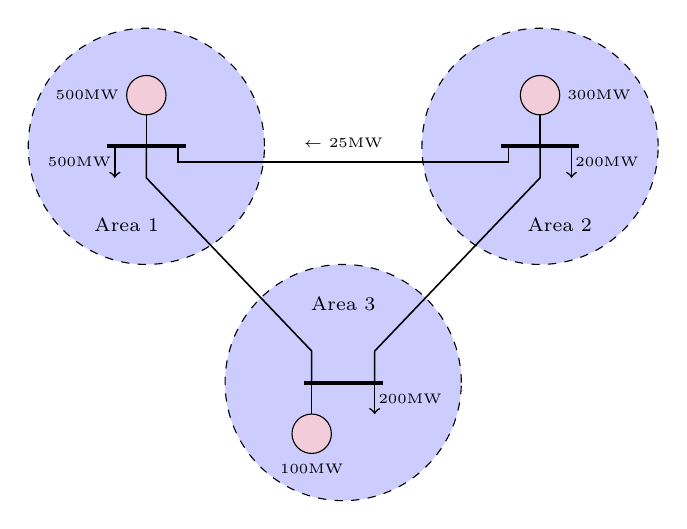
\begin{tikzpicture}
	
	% Area 1
	\draw [dashed, fill=blue!20] (0.5,0) circle (1.5cm);
		
	% Area 2
	\draw [dashed, fill=blue!20] (5.5,0) circle (1.5cm);
	
	% Area 3
	\draw [dashed, fill=blue!20] (3,-3) circle (1.5cm);
	
	% Area labels
	\node at (0.25,-1) {\scriptsize Area 1};
	\node at (5.75,-1) {\scriptsize Area 2};
	\node at (3,-2) {\scriptsize Area 3};
	
	% Bus 1
	\draw [line width=0.5mm] (0,0) -- (1,0);
	\draw [line width=0.2mm] (0.5,0) -- (0.5,0.4);
	
	% Load 1
	\draw [->, line width=0.2mm] (0.1,0) -- (0.1,-0.4);
	\node at (-0.35,-0.2) {\tiny 500MW};
	
	% Gen 1
	\draw [fill=purple!20] (0.5,0.65) circle (0.25cm);
	\node at (-0.25,0.65) {\tiny 500MW};
	
	% Bus 2
	\draw [line width=0.5mm] (5,0) -- (6,0);
	\draw [line width=0.2mm] (5.5,0) -- (5.5,0.4);
	
	% Load 2
	\draw [->, line width=0.2mm] (5.9,0) -- (5.9,-0.4);
	\node at (6.35,-0.2) {\tiny 200MW};
	
	% Gen 2
	\draw [fill=purple!20] (5.5,0.65) circle (0.25cm);
	\node at (6.25,0.65) {\tiny 300MW};
	
	% Bus 3
	\draw [line width=0.5mm] (2.5,-3) -- (3.5,-3);
	\draw [line width=0.2mm] (2.6,-3) -- (2.6,-3.4);
	
	% Load 3
	\draw [->, line width=0.2mm] (3.4,-3) -- (3.4,-3.4);
	\node at (3.85,-3.2) {\tiny 200MW};
	
	% Gen 3
	\draw [fill=purple!20] (2.6,-3.65) circle (0.25cm);
	\node at (2.6,-4.1) {\tiny 100MW};
	
	% Tie line 1 to 2
	\draw [line width=0.2mm] (0.9,0) -- (0.9,-0.2) -- (5.1,-0.2) -- (5.1,0);
	
	% Tie line 1 to 3
	\draw [line width=0.2mm] (0.5,0) -- (0.5,-0.4) -- (2.6,-2.6) -- (2.6,-3);
	
	% Tie line 2 to 3
	\draw [line width=0.2mm] (5.5,0) -- (5.5,-0.4) -- (3.4,-2.6) -- (3.4,-3);
	
	% Flow from 2 to 1
	\node at (3, 0.05) {\tiny $\leftarrow$ 25MW};
	
	% Flow from 1 to 3
	
	
	% Flow from 3 to 2
	
	
	
\end{tikzpicture}